\subsection{Adaptive Multivariate Function Approximation For Cones of Functions}

Rigorous error bounds for numerical approximations typically consist of the norm of the input function, $\norm{f}$, multiplied by the norm of the error operator.  Because $\norm{f}$ is unknown,  these error bounds cannot tell us whether a prescribed error tolerance has been met.  Adaptive numerical algorithms typically use heuristic, data-driven error bounds.  We do not know when they can be trusted.

This project is to investigate adaptive function approximation algorithms based on rigorous, data-driven error bounds.  Each algorithm assumes that the function to be approximated lies in a \emph{candidate cone}, $\cc$.  ``Candidate'' refers to functions that our algorithm can approximate accurately.  The definition of $\cc$ formalizes the idea that \emph{what we observe is nearly what we get}.  By the definition of ``cone'', if $f$ lies in $\cc$, then so does any constant multiple of $f$.  Although there are no data-driven sufficient conditions for a function to lie in $\calc$, we can specify data-driven \emph{necessary} conditions.

Our numerical approximation is the minimum norm interpolant in a reproducing kernel Hilbert space (RKHS).  Baking into $\cc$ the assumption that the norm of a function is not arbitrarily larger than the norm of its interpolant allows us to construct a rigorous data-driven error bound for the interpolant and an adaptive function approximation algorithm. Given a black-box input function, $f \in \cc$, and an error tolerance, $\varepsilon$, our algorithm returns the approximation $\ALG(f,\varepsilon) \in L^\infty$---defined only in terms of function values---for which 
$
\norm[\infty]{f - \ALG(f,\varepsilon)} \le \varepsilon, \forall f\in \cc.$

Without  a priori knowledge, we do not know whether our $f$ is typical for  the RKHS chosen.  We do not expect a unique RKHS for which $f$ is typical, but we want to infer a \emph{suitable} RKHS from the data.
Let $\{\calf_{\btheta} : \btheta \in \Theta\}$ be a family of RKHSs parameterized by $\btheta$.  An example is a generalization of the Gaussian kernel:
$
K_\btheta(\bt,\bx) =  \exp(-\norm[2]{\btheta \odot (\bt-\bx)}^2),
$
where $\odot$ denotes the Hadamard or term-by-term product. We highlight the dependence of the reproducing kernel and related quantities on $\btheta$.
Figure \ref{fig:GaussThPlot} displays the Gaussian reproducing kernel for $d=1$ for three different values of $\btheta = \theta$.  Under this parameterization, the kernel becomes flatter for small $\theta$ and more peaked for large $\theta$. For small $\theta$, we will face ill-conditioning problems.  \scnote{``flatter'' means ``praise'. Maybe change to ``more flat''?}

\begin{wrapfigure}{r}{0.28\textwidth}
  \begin{center}
    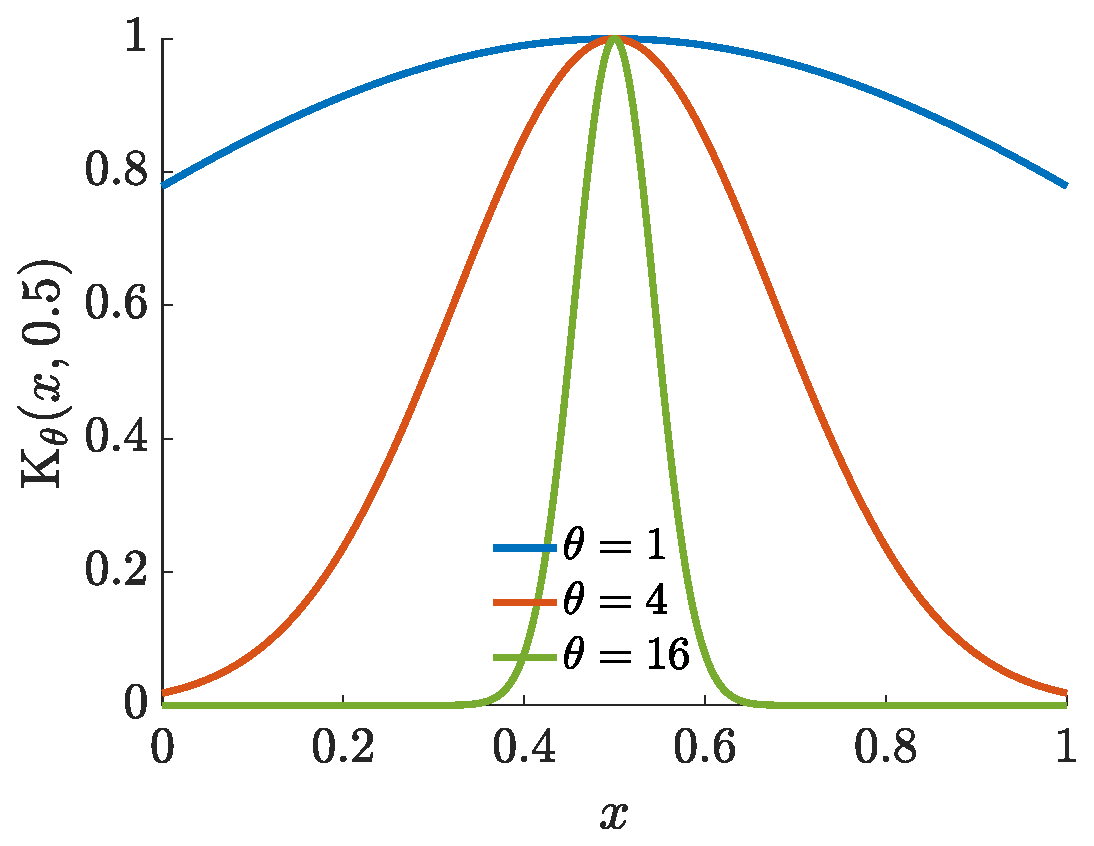
\includegraphics[width=0.25\textwidth]{KthetaPlot.eps} 
  \end{center}
  \caption{The Gaussian kernel defined above for various values of $\btheta$. \label{fig:GaussThPlot}}
\end{wrapfigure}
The goal of this project is to construct a nice candidate cone and based on that to establish an adaptive algorithm using a Gaussian kernel with the optimal parameter.
This algorithm draws upon the well-developed literature of RKHS function approximation \cite{Buh03a,Fas07a,FasMcC15a,ForFly15a,ForEtal09,RasWil06a,SchWen06a,Wah85a,Wen05a}. 
SURE students will learn the well-developed algorithms and explore a new adaptive algorithm with a nice candidate cone. 
They will also do numeric experiments to investigate the efficiency of the algorithm and how to choose the optimal parameter with different input functions.
